
\documentclass[a4paper]{article}

%\VignetteIndexEntry{BEST User Manual}

\title{Bayesian Estimation Supersedes the t-Test}
\author{John Kruschke and Mike Meredith}

\usepackage[section]{placeins}
\usepackage[usenames,dvipsnames,svgnames]{xcolor}
\usepackage[authoryear,round]{natbib}
\usepackage{graphicx, Rd}
\usepackage{float}
\usepackage{Sweave}
\usepackage[bookmarks=false]{hyperref}

\begin{document}

\maketitle


\section{Introduction}
\label{sec:intro}

The BEST package provides a Bayesian alternative to a \emph{t} test, providing much richer information about the samples and the difference in means than a simple \emph{p} value.

Bayesian estimation for two groups provides complete distributions of credible values for the effect size, group means and their difference, standard deviations and their difference, and the normality of the data. For a single group, distributions for the mean, standard deviation and normality are provided. The method handles outliers.

The decision rule can accept the null value (unlike traditional \emph{t} tests) when certainty in the estimate is high (unlike Bayesian model comparison using Bayes factors).

The package also provides methods to estimate statistical power for various research goals.

The code used for the computations is the same as that used in \citet{kruschke2012BEST}.

\textcolor{red}{TODO a suite of tests which compare package output with original output; slight problem with this is that JAGS produces slightly different output each time, so can only get maybe 2 sig.fig.}


\section{The Model}
\label{sec:model}

\begin{figure}[t]
  \centering
  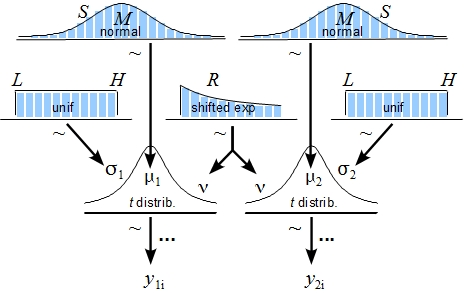
\includegraphics{figures/BESTmodel.jpg}
  \caption{\it Hierarchical diagram of the descriptive model for robust Bayesian estimation.}
  \label{fig:model}
\end{figure}

To accommodate outliers we describe the data with a distribution that has fatter tails than the normal distribution, namely the \emph{t} distribution. (Note that we are using this as a convenient description of the data, not as a sampling distribution from which \emph{p} values are derived.) The relative height of the tails of the \emph{t} distribution is governed by the shape parameter $\nu$: when $\nu$ is small, the distribution has heavy tails, and when it is large (e.g., 100), it is nearly normal. Here we refer to $\nu$ as the normality parameter.

The data (\emph{y}) are assumed to be i.d.d. draws from a \emph{t} distribution with different mean ($\mu$) and standard deviation ($\sigma$) of each population, and with a common normality parameter ($\nu$), as indicated in the lower portion of Figure~\ref{fig:model}.

The priors used are minimally informative: normal priors with large standard deviation for ($\mu$), broad uniform priors for ($\sigma$), and a shifted-exponential prior for ($\nu$), as shown in the upper part of Figure~\ref{fig:model}. Full details of the priors are given in \citet{kruschke2012BEST}.

For a general discussion see \citet{kruschke2011book}.

\section{Preparing to run BEST}
\label{sec:prepare}

BEST uses the JAGS package \citep{plummer2003} to produce samples from the posterior distribution of each parameter of interest. You will need to download JAGS from \url{http://sourceforge.net/projects/mcmc-jags/} and install it before running BEST.

BEST also requires the packages \verb@rjags@ and \verb@coda@, which should normally be installed at the same time as package BEST.

Once installed, we need to load the BEST package at the start of each \R{} session, which will also load rjags and coda and link to JAGS:
\begin{Schunk}
\begin{Sinput}
> library(BEST)
\end{Sinput}
\end{Schunk}
\begin{verbatim}
Loading required package: rjags
Loading required package: coda
Loading required package: lattice
Linked to JAGS 3.3.0
Loaded modules: basemod,bugs
\end{verbatim}



\section{An example with two groups}
\label{sec:grps2}

\subsection{Some example data}
\label{subsec:data2g}

We will use the hypothetical data from \citet{kruschke2012BEST}: ``Consider data from two groups of people who take an IQ test. Group 1 ($N_1 = 47$) consumes a ``smart drug'' while Group 2 ($N_2 = 42$) is a control group that consumes a placebo.''

\begin{Schunk}
\begin{Sinput}
> y1 = c(101,100,102,104,102,97,105,105,98,101,100,123,105,103,100,95,102,106,
         109,102,82,102,100,102,102,101,102,102,103,103,97,97,103,101,97,104,
         96,103,124,101,101,100,101,101,104,100,101)
> y2 = c(99,101,100,101,102,100,97,101,104,101,102,102,100,105,88,101,100,
         104,100,100,100,101,102,103,97,101,101,100,101,99,101,100,100,
         101,100,99,101,100,102,99,100,99)
\end{Sinput}
\end{Schunk}



\subsection{Running the model}
\label{subsec:run2g}

We run BESTmcmc and save the result in BESTout. This will take a minute or so:
\begin{Schunk}
\begin{Sinput}
> BESTout <- BESTmcmc(y1, y2, numSavedSteps = 1e+03)  ## Quick run for trials
\end{Sinput}
\end{Schunk}
\begin{verbatim}
Setting up the JAGS model...
Compiling model graph
   Resolving undeclared variables
   Allocating nodes
   Graph Size: 197
Initializing model
  |++++++++++++++++++++++++++++++++++++++++++++++++++| 100%
Burning in the MCMC chain...
  |**************************************************| 100%
Sampling final MCMC chain...
  |**************************************************| 100%
\end{verbatim}




\subsection{Basic inferences}
\label{subsec:infer2g}

The default plot (Figure~\ref{fig:means2g}) is a histogram of the posterior distribution of the difference in means. 
\begin{Schunk}
\begin{Sinput}
> plot(BESTout)
\end{Sinput}
\end{Schunk}

\begin{figure}[H]
  \centering
  \includegraphics{BEST_vig-meanDiff2grps}
  \caption{\it Default plot: posterior probability of the difference in means.}
  \label{fig:means2g}
\end{figure}

\begin{Schunk}
\begin{Sinput}
> attachBEST(BESTout)
> meanDiff <- (mu1 - mu2)
> meanDiffGTzero <- mean(meanDiff > 0)
> detachBEST()
\end{Sinput}
\end{Schunk}
Also shown is the mean of the posterior probability, which is an appropriate point estimate of the true difference in means, the 95\% Highest Density Interval (HDI), and the posterior probability that the difference is greater than zero. The 95\% HDI does not include zero, and the probability that the true value is greater than zero is shown as 99.3\%. Compare this with the output from a \emph{t} test:

\begin{Schunk}
\begin{Sinput}
> t.test(y1, y2)
\end{Sinput}
\begin{Soutput}
	Welch Two Sample t-test

data:  y1 and y2 
t = 1.6222, df = 63.039, p-value = 0.1098
alternative hypothesis: true difference in means is not equal to 0 
95 percent confidence interval:
 -0.3611848  3.4766863 
sample estimates:
mean of x mean of y 
 101.9149  100.3571 
\end{Soutput}
\end{Schunk}

Because we are dealing with a Bayesian posterior probability distribution, we can extract much more information:

\begin{itemize}
  \item We can estimate the probability that the true difference in means is above (or below) an arbitrary \emph{comparison value}. For example, the drug is claimed to increase IQ scores by at least 1.5 units.
  \item The probability that the difference in yields is precisely zero is zero. More interesting is the probability that the difference may be too small to matter. We can define a \emph{region of practical equivalence} (ROPE) around zero, and obtain the probability that the true value lies therein. For the IQ example, a difference of $\pm$~0.1 may be too small to matter.
\end{itemize}

\begin{Schunk}
\begin{Sinput}
> plot(BESTout, compVal=1.5, ROPE=c(-0.1,0.1))
\end{Sinput}
\end{Schunk}
\begin{figure}[H]
  \centering
  \includegraphics{BEST_vig-meanDiff2grpsMore}
  \caption{\it Posterior probability of the difference in means with compVal=1.5 and ROPE $\pm$~0.1.}
  \label{fig:means2gMore}
\end{figure}

The plot annotations show that the probability that the increased IQ is >~1.5 is not plausible. In this case it's clear that the effect is large, but if most of the probability mass (say, 95\%) lay within the ROPE, we would accept the null value for practical purposes.

\textcolor{red}{TODO effect size graph}

\bigskip
BEST deals appropriately with differences in standard deviations between the samples and departures from normality due to outliers. We can check the difference in standard deviations or the normality parameter with \texttt{plot} (Figure~\ref{fig:sd2g+nu2g}).
\begin{Schunk}
\begin{Sinput}
> par(mfrow=1:2)
> plot(BESTout, which="sd")
> plot(BESTout, which="nu")
\end{Sinput}
\end{Schunk}

\begin{figure}[H]
  \centering
  \includegraphics{BEST_vig-sd2grps}
  \caption{\it Posterior plots for difference in standard deviation and for the normality parameter.}
  \label{fig:sd2g+nu2g}
\end{figure}

The \texttt{summary} method gives us more information on the parameters of interest, including derived parameters:
\begin{Schunk}
\begin{Sinput}
> summary(BESTout)
\end{Sinput}
\begin{Soutput}
             mean  median    mode HDI%    HDIlo   HDIup compVal %>compVal
mu1       101.542 101.532 101.509   95 100.8998 102.217                  
mu2       100.517 100.521 100.520   95 100.0642 100.923                  
muDiff      1.026   1.018   0.944   95   0.2740   1.889       0      99.3
sigma1      2.036   2.014   2.041   95   1.3398   2.833                  
sigma2      1.049   1.040   1.042   95   0.7064   1.441                  
sigmaDiff   0.987   0.968   0.929   95   0.1994   1.782       0      99.5
nu          1.853   1.762   1.687   95   1.0147   2.771                  
log10nu     0.255   0.246   0.237   95   0.0562   0.468                  
effSz       0.649   0.631   0.564   95   0.0862   1.184       0      99.3
\end{Soutput}
\end{Schunk}

Here we have summaries of posterior distributions for the derived parameters: difference in means (\texttt{muDiff}), difference in standard deviations (\texttt{sigmaDiff}) and effect size (\texttt{effSz}). As with the plot command, we can set values for \texttt{compVal} and \textt{ROPE} for each of the parameters of interest.

\textcolor{red}{TODO show example output with compVal, ROPE}


\subsection{Checking convergence and fit}
\label{subsec:checks2g}

The output from \texttt{BESTmcmc} has class BEST, which has a \texttt{print} method:
\begin{Schunk}
\begin{Sinput}
> class(BESTout)
\end{Sinput}
\begin{Soutput}
[1] "BEST"      "mcmc.list"
\end{Soutput}
\begin{Sinput}
> print(BESTout)
\end{Sinput}
\begin{Soutput}
MCMC fit results for BEST analysis:
1002 simulations saved.
            mean     sd  median    HDIlo   HDIup  Rhat n.eff
mu[1]    101.542 0.3577 101.532 100.8998 102.217 1.002   759
mu[2]    100.517 0.2187 100.521 100.0642 100.923 1.002   572
nu         1.853 0.4778   1.762   1.0147   2.771 1.036   301
sigma[1]   2.036 0.3965   2.014   1.3398   2.833 1.016   241
sigma[2]   1.049 0.1911   1.040   0.7064   1.441 1.000   486

'HDIlo' and 'HDIup' are the limits of a 95% HDI credible interval.
'Rhat' is the potential scale reduction factor (at convergence, Rhat=1).
'n.eff' is a crude measure of effective sample size.
\end{Soutput}
\end{Schunk}

This shows the mean, standard deviation and median of the posterior distributions of the parameters in the model, together with a 95\% Highest Density Interval: see the help page for the \texttt{hdi} function for details.
Two convergence diagnostic measures are also displayed:

\begin{itemize}
  \item \texttt{Rhat} is the Brooks-Gelman-Rubin scale reduction factor, which is 1 on convergence; values between 1 and 1.02 are considered satisfactory (reference?); increase the \texttt{burnInSteps} argument to \texttt{BESTmcmc} if any of the \texttt{Rhat}s are too big.
  \item \texttt{n.eff} is the effective sample size, which is less than the number of simulations because of autocorrelation between successive values in the sample; values of \texttt{n.eff} around 10,000 are needed for stable estimates of 95\% credible intervals (reference?). If these are not satisfactory, you can increase the \texttt{numSavedSteps} or \texttt{thinSteps} arguments.
\end{itemize}

See the help pages for the \texttt{coda} package for more information. Any of the diagnostic tests in \texttt{coda} can be used with \texttt{BESTmcmc} output. (at present!!)

\bigskip
As a further check, we can compare \emph{posterior predictive distributions} with the original data:

\begin{Schunk}
\begin{Sinput}
> plotPostPred(BESTout)
\end{Sinput}
\end{Schunk}
\begin{figure}[H]
  \centering
  \includegraphics{BEST_vig-ppd2grps}
  \caption{\it Posterior predictive plots together with a histogram of the data.}
  \label{fig:ppd2g}
\end{figure}

Each panel of Figure~\ref{fig:ppd2g} corresponds to one of the samples, and shows curves produced by selecting 30 random steps in the MCMC chain and plotting the \emph{t} distibution with parameters ($\mu$), ($\sigma$) and ($\nu$) for that step. Also shown is a histogram of the actual data. We can visually assess whether the model is a reasonably good fit to the sample data.

The function \texttt{plotAll} puts histograms of all the posterior distributions and the posterior predictive plots onto a single page (Figure~\ref{fig:plotAll2g}).

\begin{Schunk}
\begin{Sinput}
> plotAll(BESTout)
\end{Sinput}
\end{Schunk}
\begin{figure}[bht]
  \label{fig:plotAll2g}
  \centering
  \includegraphics[width=0.95\textwidth]{BEST_vig-plotAll2grps}
  \caption{\it All the posterior distributions and the posterior predictive plots.}
\end{figure}



\subsection{Working with individual parameters}
\label{subsec:attach2g}

Objects of class \texttt{BEST} contain long vectors of simulated draws from the posterior distribution of each of the parameters in the model. To access these values, we attach the \texttt{BEST} object to the search path with \texttt{attachBEST}:
\begin{Schunk}
\begin{Sinput}
> attachBEST(BESTout)
\end{Sinput}
\begin{Soutput}
You can now access mu1, mu2, nu, sigma1, sigma2 by name.
\end{Soutput}
\begin{Sinput}
> length(nu)
\end{Sinput}
\begin{Soutput}
[1] 1002
\end{Soutput}
\begin{Sinput}
> meanDiff <- (mu1 - mu2)
> meanDiffGTzero <- mean(meanDiff > 0)
> meanDiffGTzero
\end{Sinput}
\begin{Soutput}
[1] 0.993014
\end{Soutput}
\end{Schunk}
For example, you may wish to look at the ratio of the variances rather than the difference in the standard deviations. You can calculate a vector of draws from the posterior distribution, calculate summary statistics, and plot the distribution with \texttt{plotPost} (Figure~\ref{fig:vars2g}):
\begin{Schunk}
\begin{Sinput}
> varRatio <- sigma1^2 / sigma2^2
> median(varRatio)
\end{Sinput}
\begin{Soutput}
[1] 3.829349
\end{Soutput}
\begin{Sinput}
> hdi(varRatio)
\end{Sinput}
\begin{Soutput}
    lower     upper 
0.9026735 8.0857808 
attr(,"credMass")
[1] 0.95
\end{Soutput}
\begin{Sinput}
> mean(varRatio > 1)
\end{Sinput}
\begin{Soutput}
[1] 0.99501
\end{Soutput}
\begin{Sinput}
> plotPost(varRatio)
\end{Sinput}
\end{Schunk}
\begin{figure}[H]
  \centering
  \includegraphics[width=0.6\textwidth]{BEST_vig-vars2grps}
  \caption{\it Posterior distribution of the ratio of the sample variances.}
  \label{fig:vars2g}
\end{figure}



\section{An example with a single group}
\label{sec:1grp}

Applying BEST to a single sample, or for differences in paired observations, works in much the same way as the two-sample method and uses the same function calls. To run the model, simply use \texttt{BESTmcmc} with only one vector of observations.
\begin{Schunk}
\begin{Sinput}
> y0 <- c(1.89, 1.78, 1.30, 1.74, 1.33, 0.89)
> BESTout1g <- BESTmcmc(y0, numSavedSteps = 1e+03)  ## Quick run for trials
\end{Sinput}
\end{Schunk}
\begin{verbatim}
Setting up the JAGS model...
Compiling model graph
   Resolving undeclared variables
   Allocating nodes
   Graph Size: 21

Initializing model

  |++++++++++++++++++++++++++++++++++++++++++++++++++| 100%
Burning in the MCMC chain...
  |**************************************************| 100%
Sampling final MCMC chain...
  |**************************************************| 100%
\end{verbatim}

This time we have a single mean and standard deviation. The default plot (Figure~\ref{fig:mean1g}) shows the posterior distribution of the mean. 
\begin{Schunk}
\begin{Sinput}
> BESTout1g
\end{Sinput}
\begin{Soutput}
MCMC fit results for BEST analysis:
1002 simulations saved.
         mean      sd  median  HDIlo   HDIup  Rhat n.eff
mu     1.4934  0.2147  1.4961 1.1120  1.9261 1.005   465
nu    31.4591 28.6672 21.9022 1.0384 90.6097 1.024   228
sigma  0.4936  0.2480  0.4314 0.1642  0.9889 1.051   222

'HDIlo' and 'HDIup' are the limits of a 95% HDI credible interval.
'Rhat' is the potential scale reduction factor (at convergence, Rhat=1).
'n.eff' is a crude measure of effective sample size.
\end{Soutput}
\begin{Sinput}
> plot(BESTout1g)
\end{Sinput}
\end{Schunk}
\begin{figure}[H]
  \centering
  \includegraphics{BEST_vig-mean1grp}
  \caption{\it Default plot: posterior probability distribution for the mean.}
  \label{fig:mean1g}
\end{figure}

Standard deviation, the normality parameter and effect size can be plotted individually, or on a single page with \texttt{plotAll} (Figure~\ref{fig:plotAll1g}).

\begin{Schunk}
\begin{Sinput}
> plotAll(BESTout1g)
\end{Sinput}
\end{Schunk}
\begin{figure}[bht]
  \centering
  \includegraphics[width=0.95\textwidth]{BEST_vig-plotAll1grp}
  \caption{\it All the posterior distributions and the posterior predictive plots.}
  \label{fig:plotAll1g}
\end{figure}

And we can access the draws from the posterior distributions after attaching them to the search path:

\begin{Schunk}
\begin{Sinput}
> attachBEST(BESTout1g)
\end{Sinput}
\begin{Soutput}
You can now access mu, nu, sigma by name.
\end{Soutput}
\begin{Sinput}
> length(nu)
\end{Sinput}
\begin{Soutput}
[1] 1002
\end{Soutput}
\begin{Sinput}
> variance <- sigma^2
> plotPost(variance)
> detachBEST()
\end{Sinput}
\end{Schunk}
\begin{figure}[H]
  \centering
  \includegraphics[width=0.6\textwidth]{BEST_vig-attach1grp}
  \caption{\it Posterior distribution of the sample variance.}
  \label{fig:var1g}
\end{figure}


\section{Power analysis}
\label{sec:power}

Power analysis seeks to answer the question: ``What is the probability that I will meet my research goals with my intended study design?'' Research goals here may be:
\begin{itemize}
  \item precision: the width of the HDI is less than a predetermined criterion;
  \item accept the null: the HDI falls entirely within the ROPE;
  \item reject the null: the HDI falls entirely outside the ROPE, either above or below it.
\end{itemize}

Of course, success depends on the real state of the populations studied, and assumptions about means, standard deviations, and normality are unavoidable. For a \emph{retrospective} power analysis, we assume that the estimates derived from a past study are correct; for a \emph{prospective} power analysis, we provide a fresh set of assumed values.

The approach used in BEST recognises uncertainty about the parameter values, and generates simulated samples based on plausible sets of values. The simulated samples are analysed using \texttt{BESTmcmc} and a tally kept of the number of simulations in which the research criteria were satisfied. The tally is used to calculate the posterior probability of meeting the criterion, and the mean and 95\% HDI of the posterior are returned.

\subsection{Retrospective power analysis}
\label{subsec:retroPower}

Retrospective power analysis makes use of the output from a previous study. We will continue the example from Section~\ref{sec:grps2}. For the difference in means, we want the 95\% HDI width to be less than 2 tonnes/ha and set the ROPE at $\pm$~0.1. By default, sample sizes match those of the original study. Running 200 simulations (the default) takes about 30 mins.

\begin{Schunk}
\begin{Sinput}
> powerRet1 <- BESTpower(BESTout, ROPEm = c(-0.1,0.1), maxHDIWm = 2.0, 
               saveName = NULL) 
\end{Sinput}
\end{Schunk}
\begin{verbatim}
:::::::::::::::::::::::::::::::::::::::::::::::::::::::::::::::
Power computation: Simulated Experiment 1 of 200 :

Setting up the JAGS model...
Compiling model graph
   Resolving undeclared variables
   Allocating nodes
   Graph Size: 197
...
After 200 Simulated Experiments, Posterior Probability
       of meeting each criterion is (mean and 95% CrI):
                      mean CrIlo CrIhi
  mean:   HDI > ROPE 0.446 0.377 0.514
  mean:   HDI < ROPE 0.005 0.000 0.015
  mean:  HDI in ROPE 0.005 0.000 0.015
  mean: HDI width ok 0.589 0.521 0.656
\end{verbatim}

We did not set criteria for standard deviation or effect size, so only the results for the mean are displayed. It is possible to plot the results for the first few simulations (cf. Figure~\ref{fig:plotAll2g}) by setting the argument \texttt{showFirstNrep} to a positive integer (\emph{Note for Mac users}: this uses X11 which is no longer included in Mac OS X 10.8. The first time you try to run it, you will be prompted to install XQuartz; it should work thereafter.) 

Retrospective power analysis for the single-sample case is implemented in the same way, but the criteria now apply to the mean or standard deviation of the sample rather than the difference between samples.


\subsection{Prospective power analysis}
\label{subsec:proPower}

This is implemented as a three-step process. For a discussion of the advantages of this procedure, see \citet{kruschke2012BEST}.

\subsubsection{Generate an idealized data set}
\label{subsec:proPower1}

The first step is to specify the means and standard deviations of two normally distributed groups, and the sample size for each group. We also specify the percentage of the simulated data that should be outliers, and the (larger) standard deviation for the outliers.

With these inputs, the function \texttt{makeData} generates (and plots) an ideal data set matching our specification:

\begin{Schunk}
\begin{Sinput}
> proData <- makeData(mu1=108, sd1=17, mu2=100, sd2=15, nPerGrp=20, 
                      pcntOut=10, sdOutMult=2.0)
\end{Sinput}
\end{Schunk}
\begin{figure}[H]
  \centering
  \includegraphics[width=0.6\textwidth]{BEST_vig-proPower1}
  \caption{\it Distribution of the idealised samples for each group (histograms), together with the true distributions of the outliers (red curve) and non-outliers (blue curve). The solid black curve is the combined distribution.}
  \label{fig:proPower1}
\end{figure}

\subsubsection{Generate plausible parameter values}
\label{subsec:proPower2}

Next we generate sets of parameter values which are plausible in view of our ideal data set. This is accomplished by \texttt{BESTmcmc}. We plan to do 200 simulations; since values tend to be highly correlated, we generate 2000 and will select 200 from these. Figure~\ref{fig:proPower2} summarized the distributions of the parameters we will use.

\begin{Schunk}
\begin{Sinput}
> proMCMC <- BESTmcmc(proData$y1, proData$y2, numSavedSteps=2000)  
> plotAll(proMCMC)
\end{Sinput}
\end{Schunk}
\begin{verbatim}
Setting up the JAGS model...
Compiling model graph
   Resolving undeclared variables
   Allocating nodes
   Graph Size: 99

Initializing model
  |++++++++++++++++++++++++++++++++++++++++++++++++++| 100%
Burning in the MCMC chain...
  |**************************************************| 100%
Sampling final MCMC chain...
  |**************************************************| 100%
\end{verbatim}
\begin{figure}[p]
  \centering
  \includegraphics[width=0.95\textwidth]{BEST_vig-proPower2}
  \caption{\it Summary plot of the parameter values to use for the power analysis.}
  \label{fig:proPower2}
\end{figure}

\subsubsection{Simulate and analyse the data sets}
\label{subsec:proPower3}

Finally, we simulate samples based on plausible parameter values and tally the number of times when our research criteria are met, much as we did with the retrospective power analysis.

\texttt{BESTpower} allows for the number of observations to vary across simulations. Suppose the number of volunteer subjects varies but averages around 100; we divide the number we have into two approximately equal groups. With 300 replicates, this takes over 3 hrs.

\begin{Schunk}
\begin{Sinput}
> nReplicates <- 200
> Nsubj <- rpois(nReplicates, 100)
> N1plan <- round(Nsubj / 2)
> N2plan <- Nsubj - N1plan
> powerPro <- BESTpower(proMCMC, N1=N1plan, N2=N2plan,
                 ROPEm=c(-1.5,1.5), ROPEsd=c(-2,2), ROPEeff=c(-0.5,0.5), 
                 maxHDIWm=15.0, maxHDIWsd=10.0, maxHDIWeff=1.0,
                 nRep=nReplicates) 
\end{Sinput}
\end{Schunk}
\begin{verbatim}
...
After 200 Simulated Experiments, Posterior Probability
       of meeting each criterion is (mean and 95% CrI):
                      mean CrIlo CrIhi
  mean:   HDI > ROPE 0.406 0.339 0.474
  mean:   HDI < ROPE 0.010 0.000 0.023
  mean:  HDI in ROPE 0.005 0.000 0.015
  mean: HDI width ok 0.495 0.426 0.564
    sd:   HDI > ROPE 0.233 0.175 0.291
    sd:   HDI < ROPE 0.030 0.009 0.053
    sd:  HDI in ROPE 0.005 0.000 0.015
    sd: HDI width ok 0.223 0.167 0.281
effect:   HDI > ROPE 0.089 0.052 0.129
effect:   HDI < ROPE 0.005 0.000 0.015
effect:  HDI in ROPE 0.074 0.040 0.111
effect: HDI width ok 0.975 0.954 0.994
\end{verbatim}



Power analysis for the single-sample case is analogous: provide values for arguments \texttt{mu1} and \texttt{sd1} in \texttt{makeData}, and put \texttt{mu1=NULL} and \texttt{sd1=NULL}.



\newpage % Probably want to remove this when finished.

\bibliographystyle{besjournals}

\bibliography{BEST}

\end{document}

